\documentclass[a4paper, 12pt]{article}
\usepackage[utf8]{inputenc}
\usepackage[warn]{mathtext}
\usepackage[russian]{babel}
\usepackage[T2]{fontenc}
\usepackage[warn]{mathtext}
\usepackage[justification=centering]{caption}

\usepackage{graphicx}
\graphicspath{ {images/} }
\usepackage{tikz}
\usepackage{pgfplots}

\usepackage{amsmath}
\usepackage{floatflt}
\usepackage[left=20mm, top=20mm, right=20mm, bottom=20mm, footskip=10mm]{geometry}

\usepackage{multicol}
\usepackage{multirow}
\setlength{\columnsep}{2cm}

\usepackage{multicol}
\setlength{\columnsep}{2cm}
\usepackage{hyperref}
\usepackage{wrapfig}

\begin{document}
	
\begin{titlepage}
	\centering
	\vspace{5cm}
	{\scshape\LARGE Московский физико-технический институт \par}
	\vspace{4cm}
	{\scshape\Large Лабораторная работа 5.4.2 \par}
	\vspace{1cm}
	{\huge\bfseries Исследование энергетического спектра $\beta$-частиц и определение их максимальной энергии при помощи магнитного спектрометра \par}
	\vspace{1cm}
	\vfill
\begin{flushright}
	{\large выполнил студент 924 группы ФОПФ}\par
	\vspace{0.3cm}
	{\LARGE Панферов Андрей}
\end{flushright}
	

	\vfill

% Bottom of the page
	Долгопрудный, 2021 г.
\end{titlepage}

\paragraph*{Цель работы:} с помощью магнитного спектрометра исследовать энергетический спектр $\beta$-частиц при распаде ядер $^{137}$Cs и определить их максимальную энергию.

\section*{Теоретическая часть}
	
	Бета-распад - самопроизвольное превращение ядер, при котором их массовое число не изменяется, а заряд увеличивается или уменьшается на единицу.
	В данной работе:
	$$^A_Z X \to ^{\ \, A}_{Z+1} X + e^- + \widetilde{\nu} .$$
	
	Величина $W(p_e)$ является плотностью вероятности. Распределение электронов по энергии может быть вычислено теоретически. Для разрешенных переходов вероятность $\beta$-распада просто пропорциональна статистическому весу.
	\begin{equation*}
		\label{eq:W}
		W(p_e)dp_e \propto p_e^2(E_m-E_e)^2 dp_e.
	\end{equation*}
	Кинетическая энергия электрона и его импульс связаны друг с другом обычной формулой:
	\begin{equation*}
		E = \sqrt{(p_ec)^2+(m_ec^2)^2}-m_ec^2
	\end{equation*}
	Выражение (\ref{eq:W}) приводит к спектру, имеющему вид широкого колокола. Кривая плавно отходит от нуля и столь же плавно, по параболе, касается оси абсцисс в области максимального импульса электронов.
	
	Дочерние ядра, возникающие в результате $\beta$-распада, нередко оказываются возбужденными. Возбужденные ядра отдают свою энергию либо излучая $\gamma$-квант, либо передавая избыток энергии одному из электронов внутренних оболочек атома. Излучаемые в таком процессе электроны имеют строго определенную энергию и называются \textit{конверсионными}.
	
	Конверсия чаще всего происходит на оболочках K и L. Ширина конверсионной линии является чисто аппаратурной -- по ней можно оценить разрешающую силу спектрометра.
	
\section*{Экспериментальная установка}
	Блок-схема установки для изучения $\beta$-спектров изображена на рис. \ref{pic1}. Радиоактивный источник $^{137}$Cs помещен внутрь откачанной трубы. Электроны, сфокусированные магнитной линзой, попадают в счетчик. В газоразрядном счетчике они инициируют газовый разряд и тем самым приводят к появлению электрических импульсов на электродах, которые затем регистрируются счетным прибором.
    
    \begin{figure}[h]
    \centering
    \begin{minipage}{.5\textwidth}
      \centering
      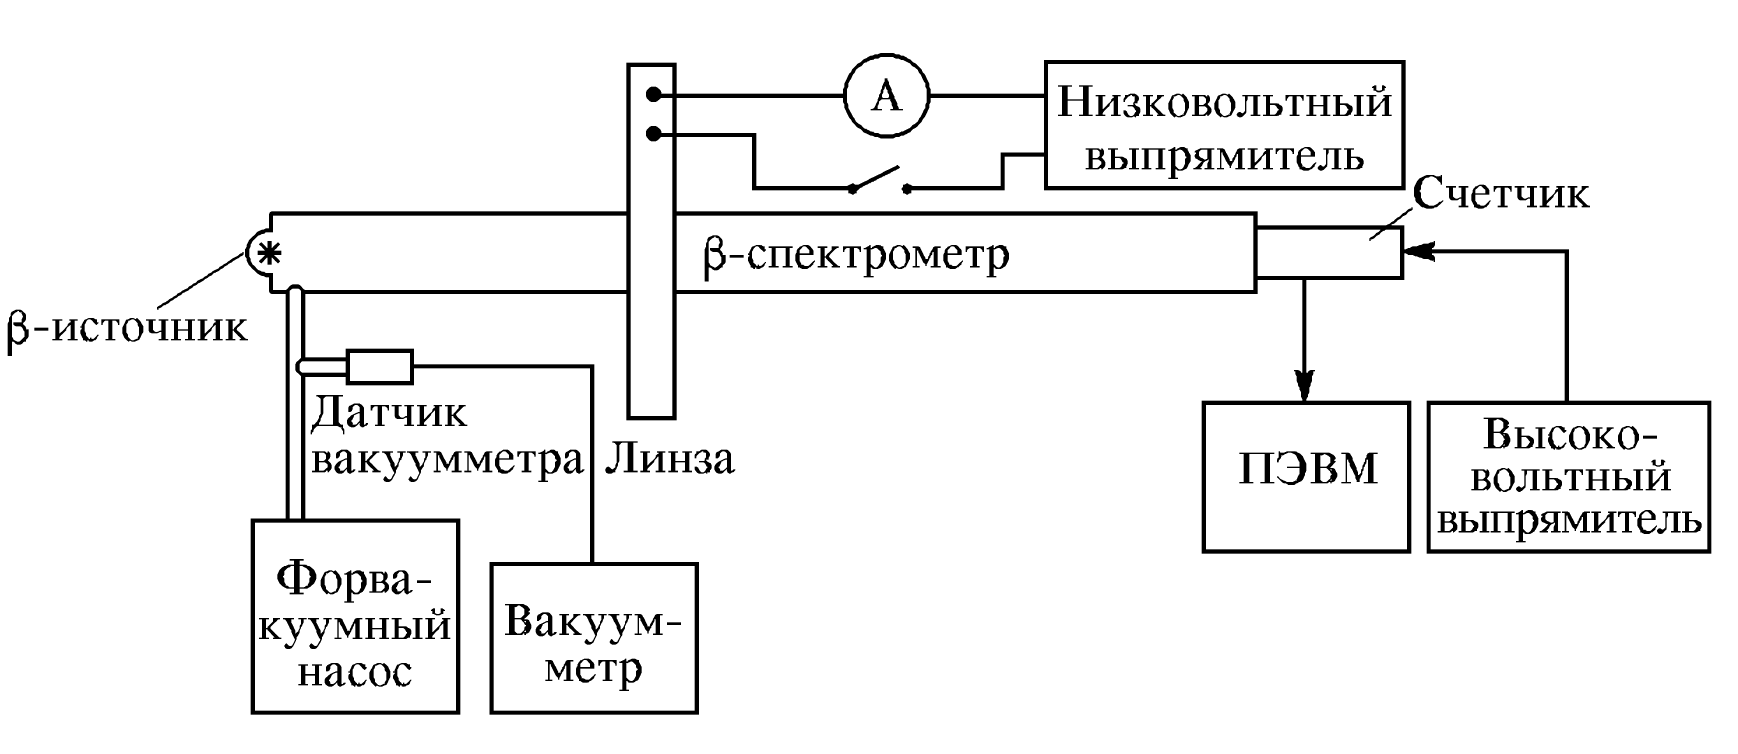
\includegraphics[width=\linewidth]{scheme.png}
      \captionof{figure}{Схема установки}
      \label{fig:test1}
    \end{minipage}%
    \begin{minipage}{.5\textwidth}
      \centering
      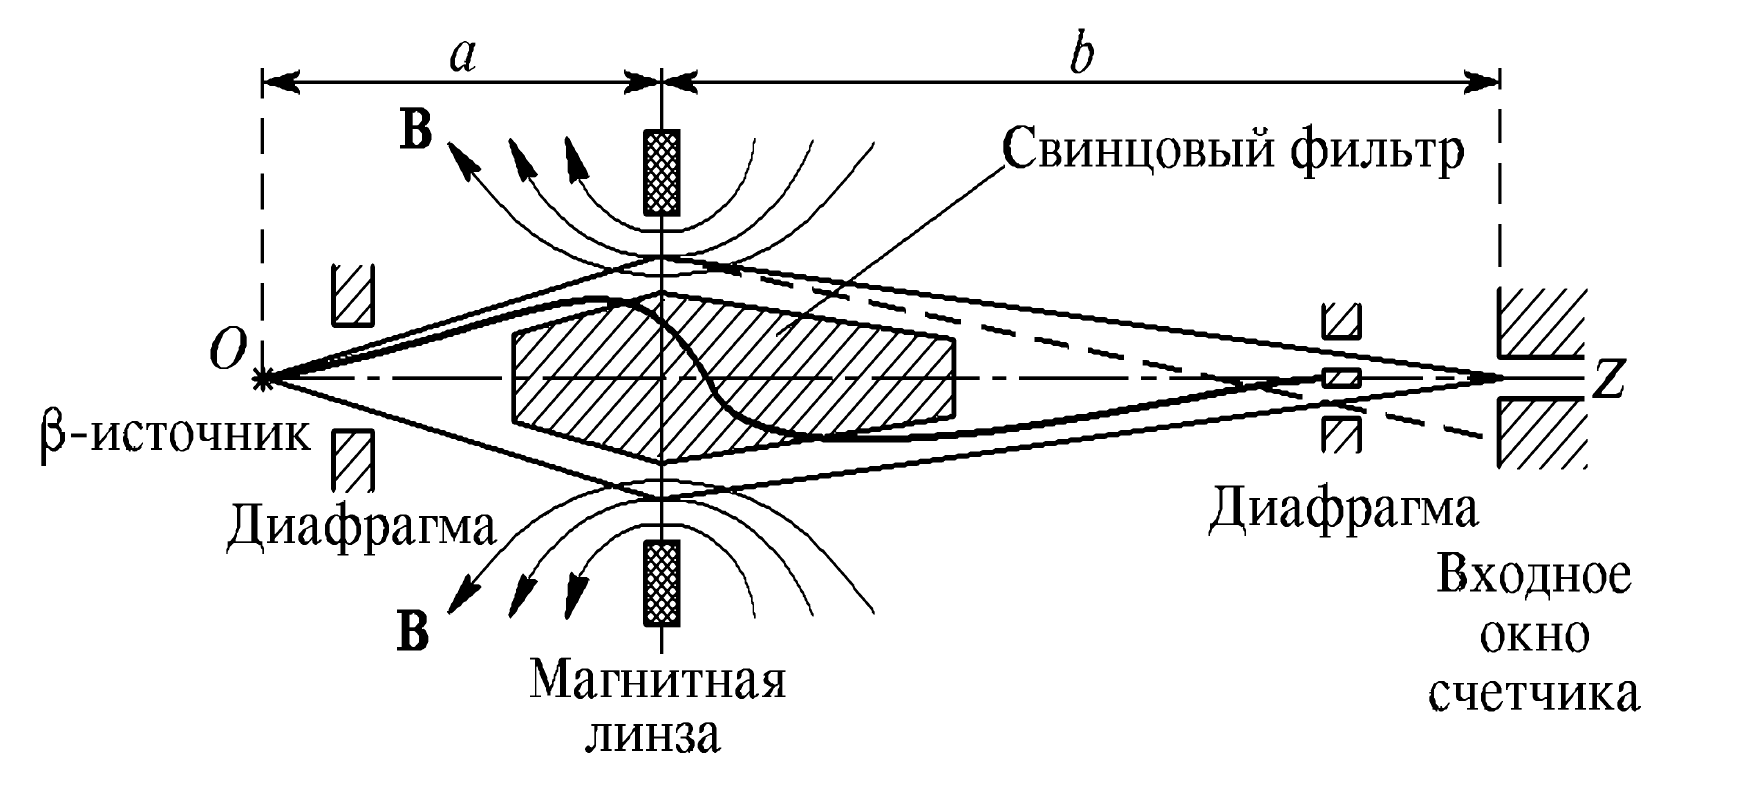
\includegraphics[width=\linewidth]{equip.png}
      \captionof{figure}{Принцип работы}
      \label{fig:test2}
    \end{minipage}
    \end{figure}
	
	Энергию $\beta$-частиц определяют с помощью $\beta$-спектрометров (рис.~\ref{pic2}). В работе используется магнитный спектрометр с <<короткой линзой>>. Отметим, что в течение всего опыта геометрия прибора остается неизменной, поэтому импульс сфокусированных электронов пропорционален величине тока:
	\begin{equation}
		\label{eq:pkI}
		\tag{$\star$}
		p_e = kI.
	\end{equation}

	Cвязь между числом частиц, регистрируемых установкой, и функцией $W(p_e)$ выражается формулой:
	\begin{equation*}
		N(p_e) \propto W(p_e)p_e,
	\end{equation*}
	откуда
	\begin{equation}
		\label{eq:fermi}
		\tag{$\star \star$}
		\frac{\sqrt{N}}{p_e^{3/2}} \propto E_m - E
	\end{equation}
	
	
	\section*{Экспериментальные данные}
		
		\begin{table}[h]
		\centering
		\caption{Результаты измерений}
		\label{table:data}
        \begin{tabular}{c|c|c|c}
        $I$, А               & $N$, 1/с               & $\sigma N$, 1/с          & $E$, кэВ          \\
        0                    & 0.50                   & 0.07                     & 0                 \\
        0.2                  & 0.59                   & 0.08                     & 29                \\
        0.4                  & 0.67                   & 0.08                     & 58                \\
        0.6                  & 0.66                   & 0.08                     & 88                \\
        0.8                  & 0.89                   & 0.09                     & 117               \\
        1                    & 0.93                   & 0.10                     & 146               \\
        1.2                  & 2.03                   & 0.15                     & 176               \\
        1.4                  & 3.01                   & 0.2                      & 206               \\
        1.6                  & 4.52                   & 0.3                      & 235               \\
        1.8                  & 6.28                   & 0.3                      & 264               \\
        2                    & 7.49                   & 0.3                      & 294               \\
        2.2                  & 8.04                   & 0.3                      & 323               \\
        2.4                  & 9.26                   & 0.4                      & 352               \\
        2.6                  & 9.53                   & 0.4                      & 382               \\
        2.8                  & 8.27                   & 0.3                      & 411               \\
        3                    & 8.04                   & 0.3                      & 440               \\
        3.2                  & 6.45                   & 0.3                      & 470               \\
        3.4                  & 4.78                   & 0.3                      & 499               \\
        3.6                  & 2.52                   & 0.2                      & 529               \\
        3.8                  & 1.68                   & 0.2                      & 558               \\
        4                    & 3.22                   & 0.2                      & 587               \\
        4.1                  & 8.25                   & 0.3                      & 602               \\
        4.15                 & 11.15                  & 0.4                      & 609               \\
        4.2                  & 13.02                  & 0.4                      & 617               \\
        4.25                 & 14.56                  & 0.4                      & 624               \\
        4.3                  & 14.31                  & 0.4                      & 631               \\
        4.35                 & 11.73                  & 0.4                      & 639               \\
        4.4                  & 10.15                  & 0.4                      & 646               \\
        4.5                  & 5.26                   & 0.3                      & 661               \\
        4.6                  & 1.97                   & 0.2                      & 675               \\
        4.8                  & 0.69                   & 0.1                      & 705               \\
        \multicolumn{2}{l}{$\sigma I = 0.02\text{А}$} & \multicolumn{2}{l}{$\sigma E = 3\text{кэВ}$}
        \end{tabular}
        \end{table}
		
		\begin{table}[h]
		    \centering
			\caption{Результаты измерения фона.}
			\label{table:exp2}
			\begin{tabular}{|c|c|c|c|}
				\hline
				$I$, A & t, с & $N_\text{ф}$, c$^{-1}$ & $\sigma_{N_\text{ф}}$, c$^{-1}$ \\ \hline
				0,00   & 100  & 1,3                    & 0,1                             \\ \hline
				4,10   & 100  & 0,54                   & 0,07                            \\ \hline
			\end{tabular}
		\end{table}
	

	\section*{Обработка результатов}
		По результатам измерений (табл.~\ref{table:data}) построим график cпектра $\beta$-распада атома $^{137}$Cs и откалибруем его. Для этого пересчитаем значения силы тока в импульс по формуле (\ref{eq:pkI}). Коэффициент $k$ определим по известной конверсионной линии:
			$$624 \ \text{кэВ} = kcI_0,$$
		где $c$ -- скорость света, $I_0 = 4,25$ А -- сила тока, при которой наблюдается конверсионный пик.
		
		\begin{figure}[h]
		    \centering
		    \begin{minipage}{0.4\textwidth}
		        \begin{tikzpicture}
                    \centering
                    \label{graph:spectrum}
                    \begin{axis}[
                        	axis lines = middle,
                        	xlabel = {$E$, кэВ},
                            ylabel = {$N$, 1/с},
                        	ylabel style={red, scale=1},
                            xlabel style={red, scale=1},
                            title style={align=left}, title={Спектр частиц},
                        	table/col sep=semicolon,
                        	error bars/x dir=both,
                            error bars/x fixed=3,
                            error bars/y dir=both,
                            error bars/y fixed relative=0.1,
                        ]
                	    \addplot +[black, only marks, error bars/.cd, x dir=both, x fixed=3,y dir=both, y explicit] table[x=E, y=N, y error=sN]{data.txt};
                	\end{axis}
                \end{tikzpicture}
		    \end{minipage}
		    \begin{minipage}{0.4\textwidth}
		        
		    \end{minipage}
		    \begin{minipage}{0.4\textwidth}
		        \begin{tikzpicture}
                    \centering
                    \label{graph:peak}
                    \begin{axis}[
                        	axis lines = middle,
                        	xlabel = {$E$, кэВ},
                            ylabel = {$\frac{\sqrt{N}}{p^{3/2}}$, единицы СИ $\cdot10^6$},
                        	ylabel style={red, scale=1},
                            xlabel style={red, scale=1},
                            title style={align=left}, title={Связь номера канала пика с углом},
                        	table/col sep=semicolon,
                        	ymin=0,
                        ]
                	    \addplot +[black, only marks, error bars/.cd, x dir=both, x fixed=3,y dir=both, y explicit] table[x=E, y=weird, y error=sweird]{data.txt};
                	    \addplot[color=red, domain=300:650]{150 - 0.245 * x};
                	\end{axis}
                \end{tikzpicture}
		    \end{minipage}
		\end{figure}

		Определим максимальную энергию $\beta$-спектра. Анализ рис.~\ref{fig:spectrum} в таком случае даст достаточно грубый результат, так как нам придётся ограничиться исследованием точек у самой верхней границы спектра. Эти точки измерены с наименьшей статистической точностью. Однако мы можем уменьшить ошибку определения максимальной энергии посредством процедуры Ферми-Кюри. Для этого мы отложим по оси ординат величину $\sqrt{N}/p^{3/2}$, а по оси абсцисс энергию $\beta$-частиц (с учётом того, что энергия электронов внутренней конверсии $^{137}$Cs равна 634 кэВ). В таком случае мы задействуем большинство экспериментальных точек, и прежде всего точки середины $\beta$-спектра, которые измерены с наилучшей точностью.
		
		Получим максимальную энергию частиц:
		
		\[E_{m} = 612\pm 7 \text{кэВ}\]
		
		
		
\section*{Обсуждение результатов и выводы}
	В ходе лабораторной работы с помощью магнитного спектрометра мы исследовали энергетический спектр $\beta$-частиц при распаде ядер $^{137}$Cs. Калибровку спектрометра осуществили по энергии электронов внутренней конверсии.
	
	Анализ графика (рис.~\ref{graph:spectrum}) показывает, что точки купола достаточно хорошо приближаются параболой. Такой вид зависимости согласуется с теоретической.
	
	Также мы определили максимальную энергию $E_m = 612 \pm 7$ кэВ вылетающих электронов при $\beta$-распаде ядра $^{137}$Cs методом Ферми-Кюри.


\end{document}